
下面详述 (7.2.364.2)。
考虑第~\ref{subsec:5-3-2} 小节的情形，
沿用该小节开头的记号。
先说明一种朴素想法遇到的困难：
若想用分叉论证证明定理~\ref{thm:5-3-14}，
可令
\[
R_{para}=\bigcup_{\rho\in[0,1]}
\{\rho\}\times
\bigl(\psi^{(1)}_\rho(L^{(1)})
\cap\psi^{(0)}_\rho(L^{(0)})\bigr).
\]
注意
$\partial R_{para}\cong
(L^{(1)\prime}\cap L^{(0)\prime})
-(L^{(1)}\cap L^{(0)})$。
于是有图式~\ref{diag:7-2-38}：

\par\medskip\noindent\begin{minipage}{\textwidth}
\centering
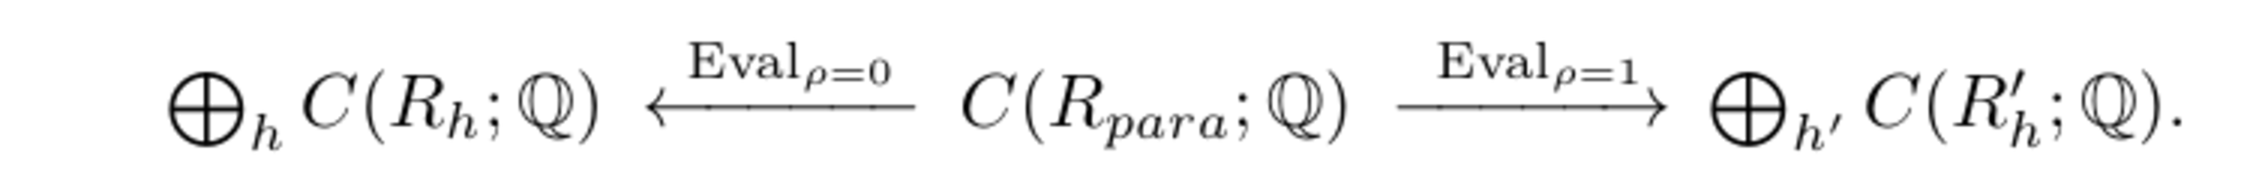
\includegraphics[width=.88\textwidth]{chapters/ch07-transversality/figures/phys-581-diagram-7-2-38-math-tight-crop.png}
\par\smallskip
{\renewcommand{\thefigure}{7.2.38}\refstepcounter{figure}
\normalfont\bfseries 图式~\thefigure\label{diag:7-2-38}}
\end{minipage}\par\medskip

或许可以尝试给图式~\ref{diag:7-2-38}
加入“量子效应”，得到图式~\ref{diag:7-2-39}：

\par\medskip\noindent\begin{minipage}{\textwidth}
\centering
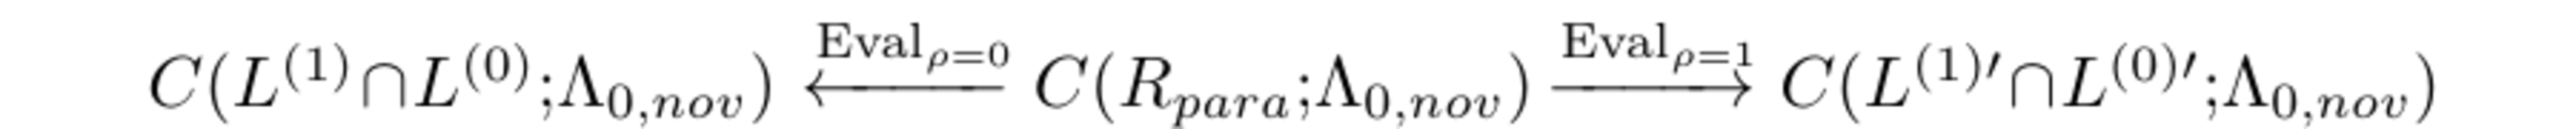
\includegraphics[width=.95\textwidth]{chapters/ch07-transversality/figures/phys-581-diagram-7-2-39-math-tight-crop.png}
\par\smallskip
{\renewcommand{\thefigure}{7.2.39}\refstepcounter{figure}
\normalfont\bfseries 图式~\thefigure\label{diag:7-2-39}}
\end{minipage}\par\medskip

然后以此证明定理~\ref{thm:5-3-14}。
但这面临两个困难：

\par\noindent\textup{(7.2.367.1)}
图式~\ref{diag:7-2-38} 中的两支箭头
在同调上不诱导同构。
因此，即便得到图式~\ref{diag:7-2-39}，
也不能直接使用定理~\ref{thm:5-2-35}。

\par\noindent\textup{(7.2.367.2)}
为了将伪全纯带的效应纳入
$C(R_{para};\Lambda_{0,\mathrm{nov}})$
的双模结构，必须考察随 $\rho$ 取并的模空间；
其中的伪全纯带连接
\[
p,q\in\psi^{(1)}_\rho(L^{(1)})
\cap\psi^{(0)}_\rho(L^{(0)}).
\]
但对于某些 $\rho$，
$\psi^{(1)}_\rho(L^{(1)})$
与 $\psi^{(0)}_\rho(L^{(0)})$
可能不横截。换言之，交点集会在某些 $\rho$
处发生分叉；这时伪全纯带的模空间更难研究。

弗洛尔在 \textbf{[Flo88IV]} 中已研究
(7.2.367.2) 的问题，
所需分析细节在 \textbf{[Lee01]} 中
有更详尽的论述。
然而，这方面尚未达到本书所需的程度：
由两个或更多变量参数化的哈密顿微分同胚族，
其情形仍未得到充分处理。
这样的族在研究同伦的同伦等问题时自然出现。

至于 (7.2.367.1)，作者目前还不知道如何处理。
我们认为，上述问题本身值得研究，
也会对弗洛尔理论今后的应用有益，
但本书不再继续讨论。

下面转而说明一种结合分叉论证与配边论证的方法。\liftIndexRangeStart{I386}
由此得到的弱滤过 $A_\infty$ 双模同态，
是相对于本小节以分叉法定义的一对
滤过 $A_\infty$ 同态而言的。

沿用第~\ref{subsec:5-3-2} 小节的记号，
令 $\{J_{\tau,t}\}_{\tau,t}$
为该小节引入的殆复结构双参数族，
并置 $J_{\rho,t}=J_{\chi^{-1}(\rho),t}$；
这里 $\chi$ 如 (5.3.2) 所述。
利用 $\{J_{\rho,i}\}_\rho$，
对 $i=0,1$ 定义图式~\ref{diag:7-2-40}：

\par\medskip\noindent\begin{minipage}{\textwidth}
\centering
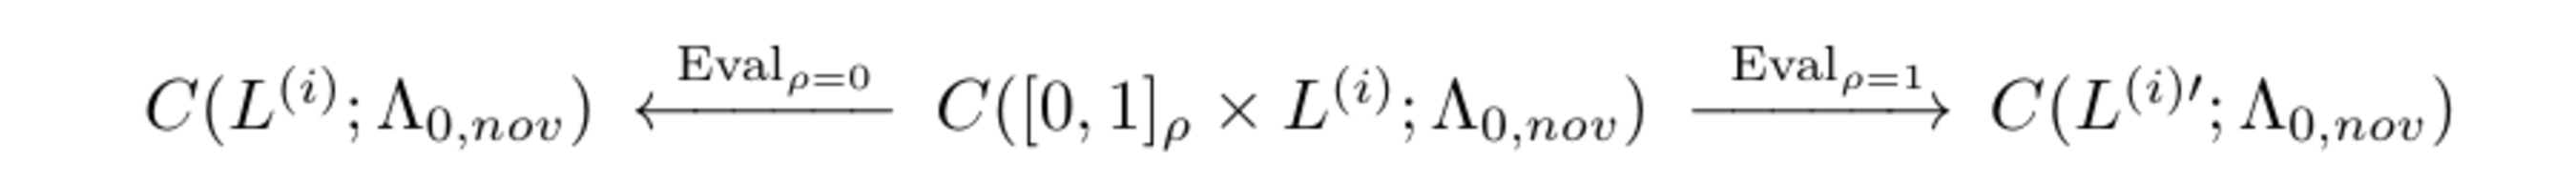
\includegraphics[width=.95\textwidth]{chapters/ch07-transversality/figures/phys-582-diagram-7-2-40-math-tight-crop.png}
\par\smallskip
{\renewcommand{\thefigure}{7.2.40}\refstepcounter{figure}
\normalfont\bfseries 图式~\thefigure\label{diag:7-2-40}}
\end{minipage}\par\medskip

严格说来，须先证明其 $A_{n,K}$ 版本，
再像前面各小节那样构造 $A_\infty$ 版本；
由于这一过程已反复进行，这里省略。

利用两端评价同态
$\operatorname{Eval}_{\rho=i}$（$i=0,1$），
将
$C(L^{(1)},L^{(0)};\Lambda_{0,\mathrm{nov}})$
和
$C(L^{(1)\prime},L^{(0)\prime};
\Lambda_{0,\mathrm{nov}})$
都视为定义在
$C([0,1]_\rho\times L^{(0)};
\Lambda_{0,\mathrm{nov}})$--
$C([0,1]_\rho\times L^{(1)};
\Lambda_{0,\mathrm{nov}})$
上的滤过 $A_\infty$ 双模。
我们将构造弱滤过 $A_\infty$ 双模同态
\begin{equation}
\begin{aligned}
C(L^{(1)}\cap L^{(0)};
\Lambda_{0,\mathrm{nov}})
\longrightarrow
C(L^{(1)\prime}\cap L^{(0)\prime};
\Lambda_{0,\mathrm{nov}}),
\end{aligned}
\tag{7.2.368}\label{eq:7-2-368}
\end{equation}
它定义在上述两个区间链代数之上。

为构造 (7.2.368)，
我们使用一个与第~\ref{subsec:5-3-4}
小节所用者略有不同的模空间。
先考虑注~\ref{rem:5-3-22} 后引入的模空间
\begin{equation}
\begin{aligned}
\overset{\circ}{\mathcal M}_{k_1,k_0}\bigl(
&(L^{(1)},\psi^{(1)}),
(L^{(0)},\psi^{(0)});\\
&\{J_{\tau,t}\}_{\tau,t};
[h,w],[h',w'];\operatorname{top}(\tau)
\bigr).
\end{aligned}
\tag{7.2.369}\label{eq:7-2-369}
\end{equation}
下面将它紧化为
\begin{equation}
\begin{aligned}
\mathcal M^{\operatorname{twp}(\tau)}_{k_1,k_0}
\bigl(\{J_{\tau,t}\}_{\tau,t};
[h,w],[h',w'];\operatorname{top}(\tau)\bigr).
\end{aligned}
\tag{7.2.370}\label{eq:7-2-370}
\end{equation}
注意，第~\ref{subsec:5-3-4} 小节使用的模空间
\begin{equation}
\begin{aligned}
\mathcal M_{k_1,k_0}\bigl(
&(L^{(1)},\psi^{(1)}),
(L^{(0)},\psi^{(0)});\\
&\{J_{\tau,t}\}_{\tau,t};
[h,w],[h',w'];\operatorname{top}(\tau)
\bigr)
\end{aligned}
\tag{7.2.371}\label{eq:7-2-371}
\end{equation}
并不是 (7.2.369) 的紧化，
因为 (7.2.369) 一般并不在其中稠密。

\begin{definition}{7.2.372}\label{def:7-2-372}
(7.2.370) 所表示的空间，
由 (7.2.371) 中满足
$\chi^{-1}(\rho_a)=\tau_a$
（对所有 $a$）的元素组成。
\end{definition}

下面说明紧化 (7.2.370)。
(7.2.371) 的一个元素可视为
一条包含于 (7.2.370) 的伪全纯带
（其中 $k_i$ 和 $w'$ 可能不同），
再加上圆盘气泡及向 $\tau\to\pm\infty$
滑移的分量。
每个圆盘气泡分量 $\Sigma_a$
都对应一个时间分配 $\rho_a$。
假定 $\chi^{-1}(\rho_a)$ 不大于
该圆盘气泡 $\Sigma_a$ 所附着之点
$(\tau_a,i)\in\mathbb R\times\{0,1\}$
的 $\mathbb R$ 分量 $\tau_a$。
这一元素属于 (7.2.370) 的必要条件是：
对所有 $a$ 均有
$\chi^{-1}(\rho_a)=\tau_a$。
